\documentclass[11pt]{article}
\usepackage{bbm}
% \usepackage{subcaption}
\def\showauthornotes{1}
\def\showkeys{0}
\def\showdraftbox{0}
\let\pref=\prettyref

\title{CSC 2240 Report: Spectral Partitioning Works: Planar graphs and finite element meshes}
\author{Chenhao Jiang, Qidong Su}
\date{December 2022}

%% Shamelessly adapted from a scribe template by Sanjeev Arora

%%%%%%%%%%%%%% Packages
% \usepackage[active,tightpage]{preview}
% \renewcommand{\PreviewBorder}{1in}
\usepackage{algorithmicx}
\usepackage{algorithm} %ctan.org\pkg\algorithms
\usepackage[noend]{algpseudocode}
\usepackage{amsfonts}
\usepackage{amsmath}
\usepackage{amssymb}
\usepackage{amstext}
\usepackage{amsthm}
\usepackage{bbm}
\usepackage{bm}
\usepackage{booktabs}
\usepackage[small]{caption}
\usepackage{color}
\usepackage{commath}
\usepackage{comment} 
\usepackage{enumerate}
\usepackage{enumitem}
\usepackage{epsfig} 
\usepackage{fancybox}
\usepackage{fullpage}
\usepackage{graphicx}
\usepackage{hyperref}
\usepackage{ifthen}
\usepackage{latexsym}
\usepackage{mdframed}
\usepackage{nicefrac}
\usepackage{pdfsync}
\usepackage{stmaryrd}
% \usepackage{subfigure}
\usepackage{subcaption}
\usepackage{tabularx}
\usepackage{textcomp}
\usepackage{thm-restate}
\usepackage{thmtools}
\usepackage{url}
\usepackage{verbatim}
\usepackage{wrapfig}
% \usepackage{xspace}


%%%%%%%%%%%%%% Use for definitions
\newcommand{\defeq}{\stackrel{\textup{def}}{=}}
\DeclareMathOperator{\vol}{\mathsf{vol}}
\DeclareMathOperator{\schur}{\mathsf{schur}}


%%%%%%%%%%%%%% Theorem Environments
\newtheorem{theorem}{Theorem}[section]
\newtheorem{problem}{Problem}
\newtheorem{lemma}[theorem]{Lemma}
\newtheorem{corollary}[theorem]{Corollary}
\newtheorem{conjecture}[theorem]{Conjecture}
\newtheorem{observation}[theorem]{Observation}
\newtheorem{proposition}[theorem]{Proposition}

\newtheorem{fact}[theorem]{Fact}
\newtheorem{claim}[theorem]{Claim}
\newtheorem{assumption}[theorem]{Assumption}
%\newtheorem{warning}[theorem]{Warning}

\theoremstyle{definition}
\newtheorem{definition}[theorem]{Definition}
\newtheorem{remark}[theorem]{Remark}


\newcommand{\eps}{\varepsilon}



\newenvironment{fminipage}%
  {\begin{Sbox}\begin{minipage}}%
  {\end{minipage}\end{Sbox}\fbox{\TheSbox}}

\newenvironment{algbox}[0]{\vskip 0.2in
\noindent 
\begin{fminipage}{6.3in}
}{
\end{fminipage}
\vskip 0.2in
}

%%%%%%%%%%%%%% Probability stuff
\DeclareMathOperator*{\pr}{\bf Pr}
\DeclareMathOperator*{\av}{\mathbbm{E}}
\DeclareMathOperator*{\var}{\bf Var}

% \newcommand\pr{\mathop{\mbox{\bf Pr}}}
% \newcommand\av{\mathop{\mbox{\bf E}}}
% \newcommand\var{\mathop{\mbox{\bf Var}}}

%%%%%%%%%%%%%% Matrix stuff
\newcommand{\tr}[1]{\mathop{\mbox{Tr}}\left({#1}\right)}
\newcommand{\diag}[1]{{\bf Diag}\left({#1}\right)}

%% Notation for integers, natural numbers, reals, fractions, sets, cardinalities
%%and so on
\newcommand{\nfrac}[2]{\nicefrac{#1}{#2}}
\def\abs#1{\left| #1 \right|}
\renewcommand{\norm}[1]{\ensuremath{\left\lVert #1 \right\rVert}}

\newcommand{\floor}[1]{\left\lfloor\, {#1}\,\right\rfloor}
\newcommand{\ceil}[1]{\left\lceil\, {#1}\,\right\rceil}

\newcommand{\pair}[1]{\left\langle{#1}\right\rangle} %for inner product

\newcommand\B{\{0,1\}}      % boolean alphabet  use in math mode
\newcommand\bz{\mathbb Z}
\newcommand\nat{\mathbb N}
\newcommand\rea{\mathbb R}
\newcommand\com{\mathbb{C}}
\newcommand\plusminus{\{\pm 1\}}
\newcommand\Bs{\{0,1\}^*}   % B star use in math mode

\newcommand{\V}[1]{\mathbf{#1}} % Used to denote bold commands
                                % e.g. vectors, matrices
\DeclareRobustCommand{\fracp}[2]{{#1 \overwithdelims()#2}}
\DeclareRobustCommand{\fracb}[2]{{#1 \overwithdelims[]#2}}
\newcommand{\marginlabel}[1]%
{\mbox{}\marginpar{\it{\raggedleft\hspace{0pt}#1}}}
\newcommand\card[1]{\left| #1 \right|} %cardinality of set S; usage \card{S}
\renewcommand\set[1]{\left\{#1\right\}} %usage \set{1,2,3,,}
\renewcommand\complement{\ensuremath{\mathsf{c}}}
% \newcommand\poly{\mbox{poly}}  %usage \poly(n)
\DeclareMathOperator{\poly}{poly}

\newcommand{\comp}[1]{\overline{#1}}
\newcommand{\smallpair}[1]{\langle{#1}\rangle}
\newcommand{\ol}[1]{\ensuremath{\overline{#1}}\xspace}

%%%%%%%%%%%%%% Mathcal shortcuts
\newcommand\calA{\mathcal{A}}
\newcommand\calB{\mathcal{B}}
\newcommand\calC{\mathcal{C}}
\newcommand\calD{\mathcal{D}}
\newcommand\calE{\mathcal{E}}
\newcommand\calF{\mathcal{F}}
\newcommand\calG{\mathcal{G}}
\newcommand\calH{\mathcal{H}}
\newcommand\calI{\mathcal{I}}
\newcommand\calJ{\mathcal{J}}
\newcommand\calK{\mathcal{K}}
\newcommand\calL{\mathcal{L}}
\newcommand\calM{\mathcal{M}}
\newcommand\calN{\mathcal{N}}
\newcommand\calO{\mathcal{O}}
\newcommand\calP{\mathcal{P}}
\newcommand\calQ{\mathcal{Q}}
\newcommand\calR{\mathcal{R}}
\newcommand\calS{\mathcal{S}}
\newcommand\calT{\mathcal{T}}
\newcommand\calU{\mathcal{U}}
\newcommand\calV{\mathcal{V}}
\newcommand\calW{\mathcal{W}}
\newcommand\calX{\mathcal{X}}
\newcommand\calY{\mathcal{Y}}
\newcommand\calZ{\mathcal{Z}}

%%%%%%%%%%%%%% {{{ authornotes }}}
\definecolor{Mygray}{gray}{0.8}

 \ifcsname ifcommentflag\endcsname\else
  \expandafter\let\csname ifcommentflag\expandafter\endcsname
                  \csname iffalse\endcsname
\fi

\ifnum\showauthornotes=1
\newcommand{\todo}[1]{\colorbox{Mygray}{\color{red}#1}}
\else
\newcommand{\todo}[1]{}
\fi

\ifnum\showauthornotes=1
\newcommand{\Authornote}[2]{{\sf\small\color{red}{[#1: #2]}}}
\newcommand{\Authoredit}[2]{{\sf\small\color{red}{[#1]}\color{blue}{#2}}}
\newcommand{\Authorcomment}[2]{{\sf \small\color{gray}{[#1: #2]}}}
\newcommand{\Authorfnote}[2]{\footnote{\color{red}{#1: #2}}}
\newcommand{\Authorfixme}[1]{\Authornote{#1}{\textbf{??}}}
\newcommand{\Authormarginmark}[1]{\marginpar{\textcolor{red}{\fbox{%\Large
#1:!}}}}
\else
\newcommand{\Authornote}[2]{}
\newcommand{\Authoredit}[2]{}
\newcommand{\Authorcomment}[2]{}
\newcommand{\Authorfnote}[2]{}
\newcommand{\Authorfixme}[1]{}
\newcommand{\Authormarginmark}[1]{}
\fi


%%%%%%%%%%%%%% Logical operators
\newcommand\true{\mbox{\sc True}}
\newcommand\false{\mbox{\sc False}}
\def\scand{\mbox{\sc and}}
\def\scor{\mbox{\sc or}}
\def\scnot{\mbox{\sc not}}
\def\scyes{\mbox{\sc yes}}
\def\scno{\mbox{\sc no}}

%% Parantheses
\newcommand{\paren}[1]{\left({#1}\right)}
\newcommand{\sqparen}[1]{\left[{#1}\right]}
\newcommand{\curlyparen}[1]{\left\{{#1}\right\}}
\newcommand{\smallparen}[1]{({#1})}
\newcommand{\smallsqparen}[1]{[{#1}]}
\newcommand{\smallcurlyparen}[1]{\{{#1}\}}

%% short-hands for relational simbols

\newcommand{\from}{:}
\newcommand\xor{\oplus}
\newcommand\bigxor{\bigoplus}
\newcommand{\logred}{\leq_{\log}}
\def\iff{\Leftrightarrow}
\def\implies{\Rightarrow}




%% macros to write pseudo-code

\newlength{\pgmtab}  %  \pgmtab is the width of each tab in the
\setlength{\pgmtab}{1em}  %  program environment
 \newenvironment{program}{\renewcommand{\baselinestretch}{1}%
\begin{tabbing}\hspace{0em}\=\hspace{0em}\=%
\hspace{\pgmtab}\=\hspace{\pgmtab}\=\hspace{\pgmtab}\=\hspace{\pgmtab}\=%
\hspace{\pgmtab}\=\hspace{\pgmtab}\=\hspace{\pgmtab}\=\hspace{\pgmtab}\=%
\+\+\kill}{\end{tabbing}\renewcommand{\baselinestretch}{\intl}}
\newcommand {\BEGIN}{{\bf begin\ }}
\newcommand {\ELSE}{{\bf else\ }}
\newcommand {\IF}{{\bf if\ }}
\newcommand {\FOR}{{\bf for\ }}
\newcommand {\TO}{{\bf to\ }}
\newcommand {\DO}{{\bf do\ }}
\newcommand {\WHILE}{{\bf while\ }}
\newcommand {\ACCEPT}{{\bf accept}}
\newcommand {\REJECT}{\mbox{\bf reject}}
\newcommand {\THEN}{\mbox{\bf then\ }}
\newcommand {\END}{{\bf end}}
\newcommand {\RETURN}{\mbox{\bf return\ }}
\newcommand {\HALT}{\mbox{\bf halt}}
\newcommand {\REPEAT}{\mbox{\bf repeat\ }}
\newcommand {\UNTIL}{\mbox{\bf until\ }}
\newcommand {\TRUE}{\mbox{\bf true\ }}
\newcommand {\FALSE}{\mbox{\bf false\ }}
\newcommand {\FORALL}{\mbox{\bf for all\ }}
\newcommand {\DOWNTO}{\mbox{\bf down to\ }}


\let\originalleft\left
\let\originalright\right
\renewcommand{\left}{\mathopen{}\mathclose\bgroup\originalleft}
  \renewcommand{\right}{\aftergroup\egroup\originalright}



\def\pleq{\preccurlyeq}
\def\pgeq{\succcurlyeq}
\def\pge{\succ}
\def\ple{\prec}

\def\Approx#1{\approx_{#1}}

\def\Span#1{\textbf{Span}\left(#1  \right)}
\def\bvec#1{{\mbox{\boldmath $#1$}}}


\def\prob#1#2{\mbox{Pr}_{#1}\left[ #2 \right]}
\def\pvec#1#2{\vec{\mbox{P}}^{#1}\left[ #2 \right]}
\def\expec#1#2{{\mathbb{E}}_{#1}\left[ #2 \right]}
\def\var#1{\mbox{\bf Var}\left[ #1 \right]}
\newcommand{\E}{\mbox{{\bf E}}}


\def\defeq{\stackrel{\mathrm{def}}{=}}
\def\setof#1{\left\{#1  \right\}}
\def\sizeof#1{\left|#1  \right|}

\def\diag#1{\textsc{Diag}\left( #1 \right)}

\def\floor#1{\left\lfloor #1 \right\rfloor}
\def\ceil#1{\left\lceil #1 \right\rceil}

\def\dim#1{\mathrm{dim} (#1)}
\def\sgn#1{\mathrm{sgn} (#1)}

\def\union{\cup}
\def\intersect{\cap}
\def\Union{\bigcup}
\def\Intersect{\bigcap}

\def\abs#1{\left|#1  \right|}

\def\norm#1{\left\| #1 \right\|}
\def\smallnorm#1{\| #1 \|}



\newcommand\Ppsi{\boldsymbol{\mathit{\Psi}}}
\newcommand\PPsi{\boldsymbol{\mathit{\Psi}}}
\newcommand\ppsi{\boldsymbol{\mathit{\psi}}}
\newcommand\pphi{\boldsymbol{\mathit{\phi}}}
\newcommand\Llambda{\boldsymbol{\mathit{\Lambda}}}
\newcommand\PPi{\boldsymbol{\Pi}}

\newcommand\ppi{\boldsymbol{\pi}}
\newcommand\cchi{\boldsymbol{\chi}}
\newcommand\aalpha{\boldsymbol{\alpha}}
\newcommand\bbeta{\boldsymbol{\beta}}
\newcommand\ggamma{\boldsymbol{\gamma}}
\newcommand\ddelta{\boldsymbol{\delta}}
\newcommand\ttau{\boldsymbol{\tau}}

\def\aa{\pmb{\mathit{a}}}
\newcommand\bb{\boldsymbol{\mathit{b}}}
\newcommand\cc{\boldsymbol{\mathit{c}}}
\newcommand\dd{\boldsymbol{\mathit{d}}}
\newcommand\ee{\boldsymbol{\mathit{e}}}
\newcommand\ff{\boldsymbol{\mathit{f}}}

\let\ggreater\gg

\renewcommand\gg{\boldsymbol{\mathit{g}}}
\newcommand\hh{\boldsymbol{\mathit{h}}}
\newcommand\ii{\boldsymbol{\mathit{i}}}
\newcommand\jj{\boldsymbol{\mathit{j}}}
\newcommand\kk{\boldsymbol{\mathit{k}}}
\renewcommand\ll{\boldsymbol{\mathit{l}}}
\newcommand\pp{\boldsymbol{\mathit{p}}}
\newcommand\qq{\boldsymbol{\mathit{q}}}
\newcommand\bs{\boldsymbol{\mathit{s}}}
\newcommand\nn{\boldsymbol{\mathit{n}}}
\newcommand\rr{\boldsymbol{\mathit{r}}}
\renewcommand\ss{\boldsymbol{\mathit{s}}}
\def\tt{\boldsymbol{\mathit{t}}}
\newcommand\uu{\boldsymbol{\mathit{u}}}
\newcommand\vv{\boldsymbol{\mathit{v}}}
\newcommand\ww{\boldsymbol{\mathit{w}}}
\newcommand\yy{\boldsymbol{\mathit{y}}}
\newcommand\zz{\boldsymbol{\mathit{z}}}
\newcommand\xx{\boldsymbol{\mathit{x}}}

\newcommand\xxbar{\overline{\boldsymbol{\mathit{x}}}}
\newcommand\ddbar{\overline{\boldsymbol{\mathit{d}}}}

\renewcommand\AA{\boldsymbol{\mathit{A}}}
\newcommand\BB{\boldsymbol{\mathit{B}}}
\newcommand\CC{\boldsymbol{\mathit{C}}}
\newcommand\DD{\boldsymbol{\mathit{D}}}
\newcommand\EE{\boldsymbol{\mathit{E}}}
\newcommand\GG{\boldsymbol{\mathit{G}}}
\newcommand\II{\boldsymbol{\mathit{I}}}
\newcommand\JJ{\boldsymbol{\mathit{J}}}
\newcommand\KK{\boldsymbol{\mathit{K}}}
\newcommand\NN{\boldsymbol{\mathit{N}}}
\newcommand\MM{\boldsymbol{\mathit{M}}}
\newcommand\LL{\boldsymbol{\mathit{L}}}
\newcommand\PP{\boldsymbol{\mathit{P}}}
\newcommand\QQ{\boldsymbol{\mathit{Q}}}
\newcommand\RR{\boldsymbol{\mathit{R}}}
\renewcommand\SS{\boldsymbol{\mathit{S}}}
\newcommand\UU{\boldsymbol{\mathit{U}}}
\newcommand\WW{\boldsymbol{\mathit{W}}}
\newcommand\VV{\boldsymbol{\mathit{V}}}
\newcommand\XX{\boldsymbol{\mathit{X}}}
\newcommand\YY{\boldsymbol{\mathit{Y}}}
\newcommand\ZZ{\boldsymbol{\mathit{Z}}}


\newcommand\ffhat{\boldsymbol{\widehat{\mathit{f}}}}
\newcommand\gghat{\boldsymbol{\widehat{\mathit{g}}}}
\newcommand\rrhat{\boldsymbol{\widehat{\mathit{r}}}}
%\newcommand\rrhat{\hat{\boldsymbol{\mathit{r}}}}
\newcommand\xxhat{\boldsymbol{\widehat{\mathit{x}}}}
\newcommand\sshat{\boldsymbol{\widehat{\mathit{u}}}}

\newcommand\fftil{\boldsymbol{\widetilde{\mathit{f}}}}
\newcommand\ggtil{\boldsymbol{\widetilde{\mathit{g}}}}
\newcommand\ppsitil{\boldsymbol{\widetilde{\mathit{\psi}}}}
\newcommand\ddeltatil{\boldsymbol{\widetilde{\mathit{\delta}}}}


\newcommand\alphahat{{\widehat{{\alpha}}}}
\newcommand\ehat{{\widehat{{e}}}}
\newcommand\nhat{{\widehat{{n}}}}\newcommand\mhat{{\widehat{{m}}}}
\newcommand\that{{\widehat{{t}}}}
\newcommand\uhat{{\widehat{{u}}}}
\newcommand\vhat{{\widehat{{v}}}}
\newcommand\what{{\widehat{{w}}}}



\newcommand\Dhat{{\widehat{{\Delta}}}}
\newcommand\Dtil{{\widetilde{{\Delta}}}}
\newcommand\Dbar{{\bar{{\Delta}}}}
\newcommand\Gbar{{\overline{{G}}}}
\newcommand\Ghat{{\widehat{{G}}}}
\newcommand\Hbar{{\overline{{H}}}}
\newcommand\Hhat{{\widehat{{H}}}}
\newcommand\Htil{{\widetilde{{H}}}}
\newcommand\Vhat{{\widehat{{V}}}}

\newcommand\Ecal{{\mathcal{{E}}}}
\newcommand\Pcal{{\mathcal{{P}}}}

\newcommand{\sym}[1]{\mathrm{sym} (#1)}

\newcommand\Otil{\widetilde{O}}

\newcommand{\opt}{\textsc{Opt}}
\newcommand{\sign}[1]{\text{sign}\paren{#1}}


\newenvironment{tight_enumerate}{
\begin{enumerate}
 \setlength{\itemsep}{2pt}
 \setlength{\parskip}{1pt}
}{\end{enumerate}}
\newenvironment{tight_itemize}{
\begin{itemize}
 \setlength{\itemsep}{2pt}
 \setlength{\parskip}{1pt}
}{\end{itemize}}


\newcommand{\vone}{\boldsymbol{\mathbf{1}}}
\newcommand{\vzero}{\boldsymbol{\mathbf{0}}}


\newcommand\DDelta{\boldsymbol{\mathit{\Delta}}}
\newcommand{\etal}{\emph{et al.}}


\newcommand{\fftilde}{\boldsymbol{\widetilde{f}}}


% Theorem-type environments
% \theoremstyle{break} 
% \theoremheaderfont{\scshape}
% \theorembodyfont{\slshape}
% \newtheorem{Thm}{Theorem}[section]
% \newtheorem{Lem}[Thm]{Lemma}
% \newtheorem{Cor}[Thm]{Corollary}
% \newtheorem{Prop}[Thm]{Proposition}
% % \theoremstyle{plain} 
% % \theorembodyfont{\rmfamily} 
% \newtheorem{Ex}[Thm]{Exercise}
% \newtheorem{Exa}[Thm]{Example}
% \newtheorem{Rem}[Thm]{Remark}
% % \theorembodyfont{\itshape}
% \newtheorem{Def}[Thm]{Definition}
% \newtheorem{Conj}[Thm]{Conjecture}
% \newtheorem{Obs}[Thm]{Observation}
% \newtheorem{Ques}[Thm]{Question}
%\newenvironment{proof}{\noindent {\sc Proof:}}{$\Box$ \medskip} 
% \newenvironment{problems} % Definition of problems
%  {\renewcommand{\labelenumi}{\S\theenumi}
% 	\begin{enumerate}}{\end{enumerate}}


%%%%%%%%%%%%%%%%% Proof Environments

\def\FullBox{\hbox{\vrule width 6pt height 6pt depth 0pt}}
%
%\def\qed{\ifmmode\qquad\FullBox\else{\unskip\nobreak\hfil
%\penalty50\hskip1em\null\nobreak\hfil\FullBox
%\parfillskip=0pt\finalhyphendemerits=0\endgraf}\fi}

\def\qedsketch{\ifmmode\Box\else{\unskip\nobreak\hfil
\penalty50\hskip1em\null\nobreak\hfil$\Box$
\parfillskip=0pt\finalhyphendemerits=0\endgraf}\fi}

%\newenvironment{proof}{\begin{trivlist} \item {\bf Proof:~~}}
 %  {\qed\end{trivlist}}

\newenvironment{proofsketch}{\begin{trivlist} \item {\bf
Proof Sketch:~~}}
  {\qedsketch\end{trivlist}}

\newenvironment{proofof}[1]{\begin{trivlist} \item {\bf Proof
#1:~~}}
  {\qed\end{trivlist}}

\newenvironment{claimproof}{\begin{quotation} \noindent
{\bf Proof of claim:~~}}{\qedsketch\end{quotation}}


%%%%%%%%%%%%%%%%%%%%%%%%%%%%%%%%%%%%%%%%%%%%%%%%%%%%%%%%%%%%%%%%%%%%%%%%%%%
%%%%%%%%%%%%%%%%%%%%%%%%%%%%%%%%%%%%%%%%%%%%%%%%%%%%%%%%%%%%%%%%%%%%%%%%%%%




\newlength{\tpush}
\setlength{\tpush}{2\headheight}
\addtolength{\tpush}{\headsep}

\newcommand{\handout}[5]{
   \noindent
   \begin{center}
   \framebox{ \vbox{ \hbox to \textwidth { {\bf \coursenum\ :\  \coursename} \hfill #5 }
       \vspace{3mm}
       \hbox to \textwidth { {\Large \hfill #2  \hfill} }
       \vspace{1mm}
       \hbox to \textwidth { {\it #3 \hfill #4} }
     }
   }
   \end{center}
   \vspace*{4mm}
   \newcommand{\lecturenum}{#1}
   \addcontentsline{toc}{chapter}{Lecture #1 -- #2}
}

\newcommand{\lecturetitle}[4]{\handout{#1}{#2}{Lecturer: \courseprof
  }{Scribe: #3}{Lecture #1 : #4}}
\newcommand{\guestlecturetitle}[5]{\handout{#1}{#2}{Lecturer:
    #4}{Scribe: #3}{Lecture #1 - #5}}


%%%%%%%%%%%%%%%%%%%%%%%%%%%%%%%%%%%%%%%%%%%%%%%%%%%%%%%%%
%%% Commands to include figures


%% PSfigure

\newcommand{\PSfigure}[3]{\begin{figure}[t] 
  \centerline{\vbox to #2 {\vfil \psfig{figure=#1.eps,height=#2} }} 
  \caption{#3}\label{#1} 
  \end{figure}} 
\newcommand{\twoPSfigures}[5]{\begin{figure*}[t]
  \centerline{%
    \hfil
    \begin{tabular}{c}
        \vbox to #3 {\vfil\psfig{figure=#1.eps,height=#3}} \\ (a)
    \end{tabular}
    \hfil\hfil\hfil
    \begin{tabular}{c}
        \vbox to #3 {\vfil\psfig{figure=#2.eps,height=#3}} \\ (b)
    \end{tabular}
    \hfil}
  \caption{#4}
  \label{#5}
%  \sublabel{#1}{(a)}
%  \sublabel{#2}{(b)}
  \end{figure*}}


\newcounter{fignum}

% fig
%command to insert figure. usage \fig{name}{h}{caption}
%where name.eps is the postscript file and h is the height in inches
%The figure is can be referred to using \ref{name}
\newcommand{\fig}[3]{%
\begin{minipage}{\textwidth}
\centering\epsfig{file=#1.eps,height=#2}
\caption{#3} \label{#1}
\end{minipage}
}%


% ffigure
% Usage: \ffigure{name of file}{height}{caption}{label}
\newcommand{\ffigure}[4]{\begin{figure} 
  \centerline{\vbox to #2 {\hfil \psfig{figure=#1.eps,height=#2} }} 
  \caption{#3}\label{#4} 
  \end{figure}} 

% ffigureh
% Usage: \ffigureh{name of file}{height}{caption}{label}
\newcommand{\ffigureh}[4]{\begin{figure}[!h] 
  \centerline{\vbox to #2 {\vfil \psfig{figure=#1.eps,height=#2} }} 
  \caption{#3}\label{#4} 
  \end{figure}} 


% {{{ draftbox }}}
\ifnum\showdraftbox=1
\newcommand{\draftbox}{\begin{center}
  \fbox{%
    \begin{minipage}{2in}%
      \begin{center}%
%        \begin{Large}%
          \large\textsc{Working Draft}\\%
%        \end{Large}\\
        Please do not distribute%
      \end{center}%
    \end{minipage}%
  }%
\end{center}
\vspace{0.2cm}}
\else
\newcommand{\draftbox}{}
\fi


%% Complexity classes
\newcommand\p{\mbox{\bf P}\xspace}
\newcommand\np{\mbox{\bf NP}\xspace}
\newcommand\cnp{\mbox{\bf coNP}\xspace}
\newcommand\sigmatwo{\mbox{\bf $\Sigma_2$}\xspace}
\newcommand\ppoly{\mbox{\bf $\p_{\bf /poly}$}\xspace}
\newcommand\sigmathree{\mbox{\bf $\Sigma_3$}\xspace}
\newcommand\pitwo{\mbox{\bf $\Pi_2$}\xspace}
\newcommand\rp{\mbox{\bf RP}\xspace}
\newcommand\zpp{\mbox{\bf ZPP}\xspace}
\newcommand\bpp{\mbox{\bf BPP}\xspace}
\newcommand\ph{\mbox{\bf PH}\xspace}
\newcommand\pspace{\mbox{\bf PSPACE}\xspace}
\newcommand\npspace{\mbox{\bf NPSPACE}\xspace}
\newcommand\dl{\mbox{\bf L}\xspace}
\newcommand\ma{\mbox{\bf MA}\xspace}
\newcommand\am{\mbox{\bf AM}\xspace}
\newcommand\nl{\mbox{\bf NL}\xspace}
\newcommand\conl{\mbox{\bf coNL}\xspace}
\newcommand\sharpp{\mbox{\#{\bf P}}\xspace}
\newcommand\parityp{\mbox{$\oplus$ {\bf P}}\xspace}
\newcommand\ip{\mbox{\bf IP}\xspace}
\newcommand\pcp{\mbox{\bf PCP}}
\newcommand\dtime{\mbox{\bf DTIME}}
\newcommand\ntime{\mbox{\bf NTIME}}
\newcommand\dspace{\mbox{\bf SPACE}\xspace}
\newcommand\nspace{\mbox{\bf NSPACE}\xspace}
\newcommand\cnspace{\mbox{\bf coNSPACE}\xspace}
\newcommand\exptime{\mbox{\bf EXP}\xspace}
\newcommand\nexptime{\mbox{\bf NEXP}\xspace}
\newcommand\genclass{\mbox{$\cal C$}\xspace}
\newcommand\cogenclass{\mbox{\bf co$\cal C$}\xspace}
\newcommand\size{\mbox{\bf SIZE}\xspace}
\newcommand\sig{\mathbf \Sigma}
\newcommand\pip{\mathbf \Pi}

%%Computational problems
\newcommand\sat{\mbox{SAT}\xspace}
\newcommand\tsat{\mbox{3SAT}\xspace}
\newcommand\tqbf{\mbox{TQBF}\xspace}


\newcommand\lagrange{{\mathcal{{L}}}}


\begin{document}

\maketitle

\section{Introduction}

\subsection{Motivation}

Graph partitioning is widely used in many scientific numerical applications, such as mapping finite element calculations on parallel machines. A good partition should be able to \textbf{minimize the edge cut} while \textbf{keep the workload balanced among partitions}. A special case is a bisection, which partitions the graph into two parts differing in size by at most 1.

Spectral partitioning is a family of algorithms associated with the second smallest eigenvalue and its corresponding eigenvectors of the Laplacian matrix. In this paper, the authors give a upper bound of the size of bisections generated by spectral partitioning on two classes of graphs: 1) bounded-degree planar graphs; 2) well-shaped meshes.

We will focus on the bounded degree planar graphs in this report as the second case is a natural generalization to higher-dimensional spaces.

\subsection{Terminology}
We omit the concepts like Laplacian matrix as they're covered and commonly used in the course.

\paragraph{partition} A partition of a graph $G$ is a division of its vertices into two disjoint subsets, $A$ and $\overline{A}$.

\paragraph{bisection} A partition is a bisection when $A$ and $\overline{A}$ differ in size by at most $1$.

\paragraph{$\delta$-seperator} For $0 < \delta \leq 2$, a partition is called \textit{$\delta$-seperator} if $\min(|A|,|\overline{A}|) \geq \delta n$.

\paragraph{cut size} Let $E(A, \overline{A})$ be the set of edges with one endpoint in $A$ and the other in $\overline{A}$. The cut size is $|E(A, \overline{A})|$

\paragraph{cut ratio} $\phi(A,\overline{A})=\frac{|E(A, \overline{A})|}{\min(|A|, |\overline{A}|)}$. It is slightly different with \textit{conductance} we learned in lectures, which is  $\frac{|E(A, \overline{A})|}{\min\left(\texttt{vol}(A), \texttt{wol}(\overline{A})\right)}$

\paragraph{isoperimetric number}
$\phi(G) = \min_{|A| \leq n/2} \frac{|E(A, \overline{A})|}{|A|}$. The isoperimetric number measures how good a ratio cut one can hope to find.

\paragraph{Fiedler value and vector}
They are the second smallest eigenvalue and its corresponding eigen vector of the Laplacian matrix.

\subsection{Outline}
In Section \ref{sp} we will introduce the spectral partition algorithm minimizing the cut ratio without considering balance. Then in Section \ref{bisection}, we'll show a algorithm iteratively calling spectral partitioning to produce a bisection with small cut. In section \ref{planar}, we'll show its application on bounded-degree planar graphs.

\subsection{Spectral Partition}\label{sp}
Let $\uu = (u_1, \dots, u_n)$ be a Fiedler vector of the Laplacian of a graph $G$. The idea of spectral partitioning is to find a splitting value $s$ and partition the vertices of $G$ into the set of $i$ such that $u_i > s$ and the set such that $u_i \leq s$. We call such a partition a \textit{Fielder cut}. There are several popular choices for the splitting value $s$:

\begin{itemize}
\item bisection: $s$ is the medium of $\{u_1,\dots, u_n\}$.
\item ratio cut: $s$ is the value that gives the best ratio cut.
\item sign cut: $s=0$
\item gap cut: $s$ is a value in the largest gap in the sorted list of Fiedler vector components
\end{itemize}

In this paper, authors analyze the spectral method that uses the splitting value that achieves the best ratio cut.

The Fiedler value $\lambda_2$ is closely linked to the isoperimetric number of the graph. If $G$ is a graph on more than three nodes, then one can show
$$
\frac{\lambda_2}{2} \leq \phi(G) \leq \sqrt{\lambda_2 (2d-\lambda_2)}
$$
where $d$ is the maximum degree.

\begin{remark}
It is slightly different from Cheeger's inequality we learned in class, since it uses unnormalized Laplacian.
\end{remark}

This inequality bounds the range of the isoperimetric value $\phi(G)$ using Fiedler value $\lambda_2$. But $\phi$ only measures the lower limit of cut ratio, but not the minimum cut ratio that \textbf{can be found by spectral partitioning}. The following theorem links $\lambda_2$ with the cut ratio given by the spectral partitioning.

\begin{theorem}[Mihail\cite{mihail1989conductance}]\label{mihail}
Let $G=(V,E)$ be a graphon $n$ nodes of maximum degree $d$, let $Q$ be its Laplacian matrix, and let $\phi$ be its isoperimetric number. For any vector $\xx \in R^n$ such that $\sum_{i=1}^n x_i = 0$,
$$
\frac{\xx^\top Q \xx}{\xx^\top \xx} \geq \frac{\phi^2}{2d}
$$

Moreover, there is an $s$ so that the cut $(\{i~:~x_i \leq s\}, \{i~:~x_i > s\})$ had ratio at most $\sqrt{2d\frac{\xx^\top Q \xx}{\xx^\top\xx}}$
\end{theorem}

If we choose the $\xx$ that minimizes $\frac{\xx^\top Q \xx}{\xx^\top\xx}$, then by the definition of Rayleigh quotient, $\frac{\xx^\top Q \xx}{\xx^\top\xx} = \lambda_2$. So we can always find an $s$ so that the cut ratio is smaller than $\sqrt{2d\lambda_2}$.

\section{From Partition to Bisection}\label{bisection}

Spectral partitioning we use splits the vertices to minimize the ratio cut, but doesn't take balance into consideration. It has no guarantee about the difference in size between the two parts.

In this part, we show that given an algorithm that can find cuts of ratio $\phi$ in $G$ and its subgraphs, we can find a \textbf{bisector} of $G$ of size $O(\phi n)$.

\begin{lemma}\label{A1_lemma}
Assume that we are given an algorithm that will find a cut of ratio at most $\phi(k)$ in every $k$-node subgraph of $G$, for some monotonically decreasing function $\phi$. Then repeated application of this algorithm (as in Algorithm~\ref{alg:bisection} and Figure~\ref{fig:bisection}) can be used to find a bisection of $G$ of size at most
$$
\int_{x=1}^n \phi(x) \dif x
$$
\end{lemma}

\begin{figure}
\centering
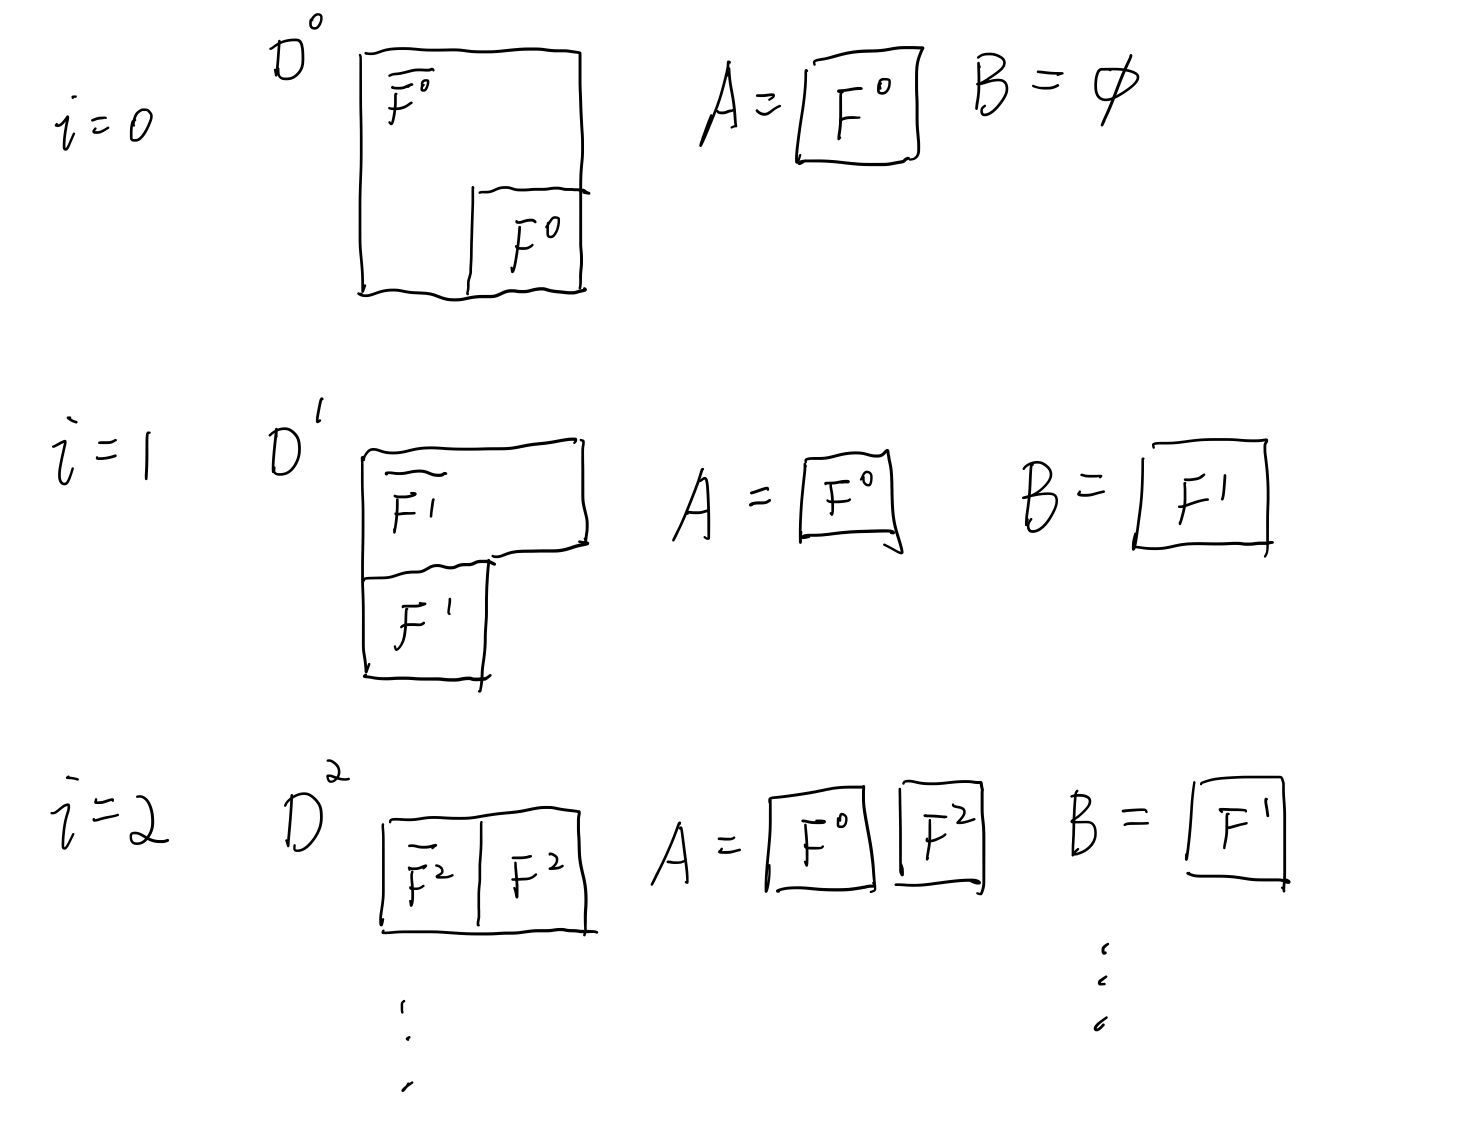
\includegraphics[width=0.6\textwidth]{figures/bisection.jpg}
\caption{Algorithm to find a bisection iteratively}
\label{fig:bisection}
\end{figure}

\begin{algorithm}
\caption{An algorithm to find a bisection}\label{alg:bisection}
\begin{algorithmic}[1]
\Require $G=(V,E)$, partition algorithm $P$ with bounded cut ratio $\phi$
\Ensure A bisection $(A, B)$ which satisfies the bound

\State $D^0 \gets G$, $A=\emptyset$, $B=\emptyset$, $i=0$
\While{$D^i \neq \emptyset$}
    \State $F^i,\overline{F^i} = P(D^i)$. Assume $|F^i| < |\overline{F^i}|$.
    \If{$|A| \leq |B|$}
        \State $A \gets A \cup F^i$
    \Else
        \State $B \gets B \cup F^i$
    \EndIf
    \State $D^{i+1} \gets \overline{F^i}$, $i \gets i+1$
\EndWhile
\end{algorithmic}
\end{algorithm}

\begin{proof}
First, we show it produces a bisection. Suppose the algorithm stops after $t$ steps. It suffices to show that for all $0 \leq t < t$, $\min(|A|, |B|) + |F^i| \leq n/2$. Because $|F^i| \leq |\overline{F^i}|$, we have 
$$
\min(|A|, |B|) + |F^i| \leq (|A| + |B| + |F^i| + |\overline{F^i}|)/2 = n/2
$$

Then we analyze the total cut size. In the $i$-th iteration, the cut ratio of $(F^i, \overline{F^i})$ is at most $\phi(|D^i|)$, so the total number of cut edges is at most

\begin{align*}
    \phi(|D^i|)|F^i| &= \sum_{j=1}^{|F^i|} \phi(|D^i|) && \text{(expand the multiplication)}\\
    &= \sum_{j=|D^i| - |F^i| + 1}^{|D^i|} \phi(|D^i|)\\
    &\leq \sum_{j=|D^i| - |F^i| + 1}^{|D^i|} \phi(j)
\end{align*}

The last inequality follows from that $\phi$ is monotonically decreasing. The total number of cut edges given by the algorithm is:

\begin{align*}
\sum_i^{t-1} \phi(|D^i|) |F^i| &\leq \sum_{i=0}^{t-1} \left( \sum_{j=|D^i| - |F^i| + 1}^{|D^i|} \phi(j) \right) \\
&= \sum_{j=1}^n \phi(j) && \text{($|D^i-1| + |F^i| = |D^i|$)} \\
&\leq \int_1^n \phi(x) \dif x && \text{($\phi$ is monotonically decreasing)}
\end{align*}

\end{proof}

\begin{remark}
If $\phi(x)=x^{-1/d}$ then 
$$
\int_i^n \phi(x) \dif x = \frac{d}{d-1} (n^{1-1/d} -1).
$$
That is $O(\phi n)$ we mentioned above.
\end{remark}

\section{Planar Graph}\label{planar}
In this part, we show that the Fiedler value of every bounded-degree planar graph is $O(1/n)$. We obtain this bound of eigenvalue by showing that every planar graph has a  good geometric embedding.  

\begin{lemma}[Embedding lemma]\label{embedding_lemma} Let $G=(V,E)$ be a graph. Then the Fiedler value of $G$, $\lambda_2$, is given by 

$$
\lambda_2 = \min \frac{\sum_{(i,j)\in E}\|\vv_i-\vv_j\|^2}{\sum_{i=1}^n\|\vv_i^2\|}
$$
where the minimum is taken over vectors $\{\vv_1,...,\vv_n\}\subset R^n$ such that 

$$
\sum_{i=1}^{n}\vv_i=\vzero
$$
where $\vzero$ denotes the zero vector.

\end{lemma}
\begin{proof}
    Because for any Laplacian matrix $L\vone=\vzero$, we know that all-ones vector is the eigenvector corresponding to the eigenvalue 0, $\lambda_2$ could be characterized as 

$$
\lambda_2 = \min \frac{\sum_{(i,j)\in E}(x_i-x_j)^2}{\sum_{i=1}^n(x_i^2)}
$$
where the minimum is taken over real $x_i$'s such that $\sum_{i=1}^{n}x_i=0$. 
(e.g.)
We then rewrite $\vv_i$ as $(v_{i,1}, ..., v_{i,n})$. For all $\{\vv_1, ..., \vv_n\}$, such that $\sum_{i=1}^{n}\vv_i=\vzero$, we have
\begin{align*}
\frac{\sum_{(i,j)\in E}\|\vv_i-\vv_j\|^2}{\sum_{i=1}^n\|\vv_i^2\|} 
& = \frac{\sum_{(i,j)\in E}\sum_{k=1}^{n}(v_{i,k}-v_{j,k})^2}{\sum_{i=1}^n\sum_{k=1}^{n}v_{i,k}^2} \\
& = \frac{\sum_{k=1}^{n}\sum_{(i,j)\in E}(v_{i,k}-v_{j,k})^2}{\sum_{k=1}^{n}\sum_{i=1}^nv_{i,k}^2} \\
\end{align*}
Since for each $k$, we have 
$$
\lambda_2 \leq \frac{\sum_{(i,j)\in E}(v_{i,k}-v_{j,k})^2}{\sum_{i=1}^nv_{i,k}^2} 
$$
therefore
$$
\lambda_2 \leq \frac{\sum_{k=1}^{n}\sum_{(i,j)\in E}(v_{i,k}-v_{j,k})^2}{\sum_{k=1}^{n}\sum_{i=1}^nv_{i,k}^2} 
$$
this follows the fact that $\sum_i x_i / \sum_i y_i \geq \min_i x_i / y_i$ for $x_i, y_i > 0$.

\end{proof}


\begin{theorem}[Koebe-Andreev-Thurston]\label{Koebe-Andreev-Thurston}. Let $G$ be a planar graph with vertex set $V=\{1,...,n\}$, and edge set $E$, there exists a set of disks $\{D_1, ...,D_n\}$ in the plane with disjoint interiors such that $D_i$ touches $D_j$ if and only if $(i,j)\in E$.
\end{theorem}
Such embedding is called a kissing disk embedding of $G$.

\begin{figure}[h]
\centering
\begin{subfigure}[b]{0.45\textwidth}
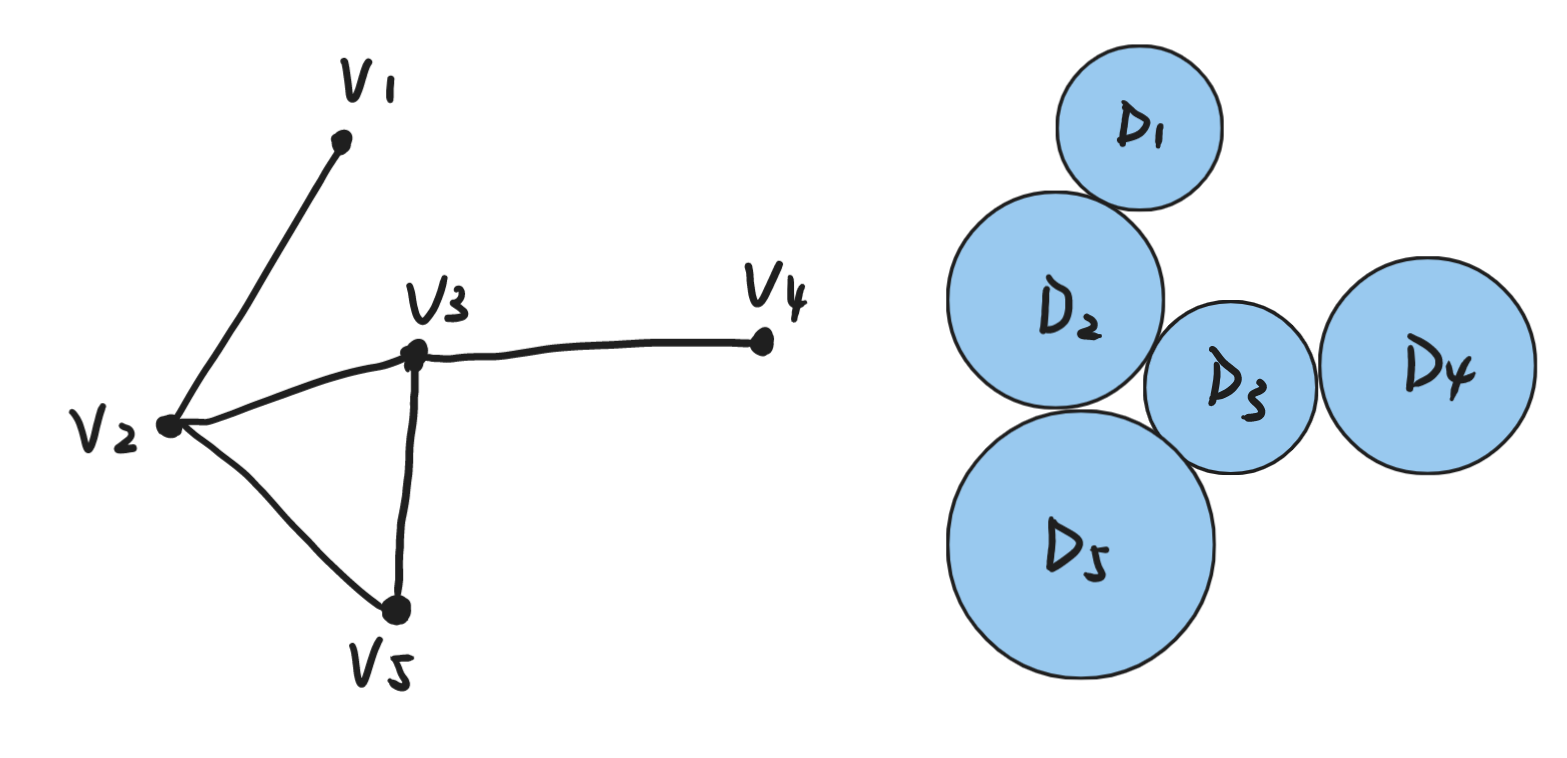
\includegraphics[width=\textwidth]{figures/kissingdisk.png}
\caption{From planar graphs to kissing disks}
\label{fig:kissing-disks}
\end{subfigure}
\hfill
\begin{subfigure}[b]{0.45\textwidth}
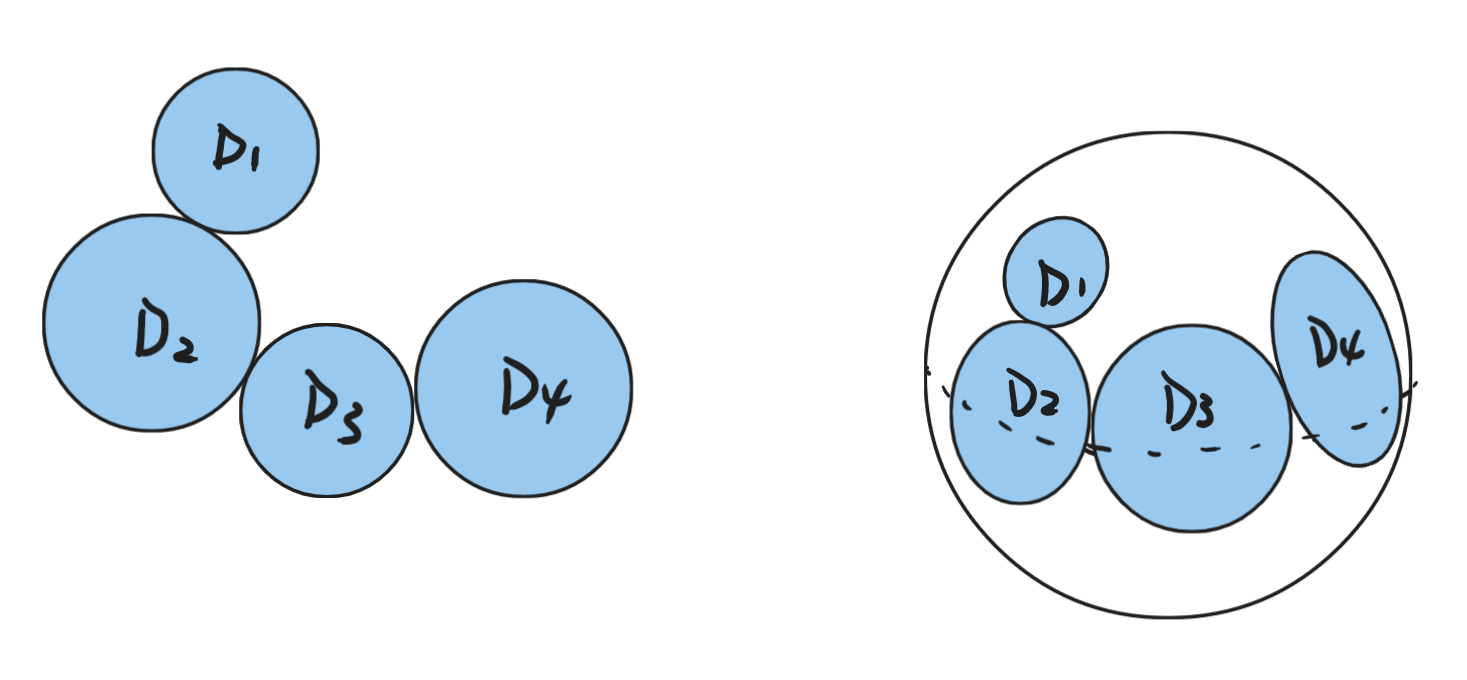
\includegraphics[width=\textwidth]{figures/kissingcaps.png}
\caption{From kissing disks to kissing caps}
\label{fig:kissing-caps}
\end{subfigure}
\caption{Kissing disks and caps}
\label{fig:kissing-disks-caps}
\end{figure}

The analogue of a disk on the sphere is a cap, which is given by the intersection of a half-space with the sphere, the boundary of which is a circle. We use stereographic projection to map the kissing disk embedding of the graph on the plane to a kissing cap embedding on the sphere. In further sections, we will show that we could always find a mapping that sends the centroid (center of gravity) of the centers of the caps to the center of the sphere.

\begin{theorem}
Let $G$ be a planar graph on $n$ nodes of degree at most $\Delta$, then the Fiedler value of $G$ is at most $\frac{16\Delta}{n}$
\end{theorem}

\begin{proof}
By theorem~\ref{Koebe-Andreev-Thurston} and theorem~\ref{th:sum_is_origin}, there is a representation of $G$ by kissing caps on the unit sphere so that the centroid of the centers of the caps is the center of the sphere. We let the center of the sphere be at the origin, and let $\vv_1,...,\vv_n$ be the centers of these caps, so that $\sum_{i=1}^{n}\vv_i=0$. As these vectors are on the unit sphere, $\|\vv_i\|=1$ for all $i$.

\begin{figure}[h]
\centering
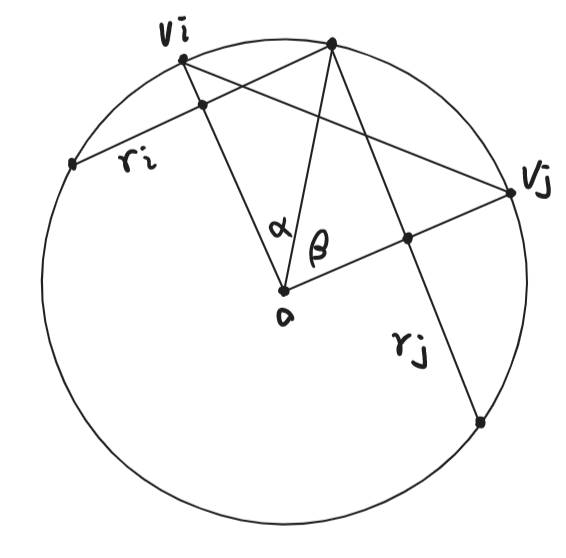
\includegraphics[width=0.3\textwidth]{figures/pmjh.png}
\label{fig:pmjh}
\caption{}
\end{figure}

 Let $r_1, ..., r_n$ be the radii of the caps, then the edge from $\vv_i$ to $\vv_j$ will have a squared length of at most $(r_i+r_j)^2 \leq 4(r_i^2 + r_j^2)$. We can prove it using elementary Euclidean geometry.
Let $r_1, ..., r_n$ be the radii of (the base of) the caps, and consider the length of $\vv_i$ to $\vv_j$ 
$\|\vv_i - \vv_j\| = 2\sin(\frac{\alpha+\beta}{2})$ \\
$r_i = \sin\alpha$, 
$r_j = \sin\beta$ \\
Let $u = \frac{\alpha +\beta}{2}, v = \frac{\alpha-\beta}{2}$, 
Consider 
\begin{align*}
\frac{r_i+r_j}{\|\vv_i - \vv_j\|}= &\frac{\sin\alpha + \sin\beta}{2\sin{\frac{\alpha+\beta}{2}}}= \frac{\sin(u+v)+sin(u-v)}{2\sin u} \\
 =&\frac{2\sin u \cos v}{2\sin u} = \cos v
\end{align*}
Since $v=\frac{\alpha-\beta}{2}$, $v$ satisfies $-\frac{\pi}{4} \leq u \leq \frac{\pi}{4}$, where $ \frac{\sqrt{2}}{2} \leq \cos v \leq 1$ always holds, and $\|\vv_i - \vv_j\| \leq \sqrt{2}(r_i + r_j)$

Consider all caps together, we have 
$$
\sum_{(i,j)\in E}\|\vv_i -\vv_j\|^2 \leq \sum_{(i,j)\in E} 2(r_i^2+r_j^2)\leq \sum_{(i,j)\in E} 4(r_i+r_j)^2 \leq 4\Delta\sum_{i=1}^{n} r_i^2
$$
as $\Delta$ is the max degree in the graph.

Since kissing caps do not overlap, the sum of the surface area of all caps is bounded by the surface area of the sphere, that is
$$
\sum_{i=1}^{n} \pi r_i^2 \leq 4\pi 
$$
therefore
$$
\sum_{(i,j)\in E}\|\vv_i -\vv_j\|^2  \leq 16\Delta
$$
Since we know that $\|\vv_i\|=1$ for all $i$, we have  $\sum_{i=1}^{n}\|\vv_i\|^2=n$, and hence
$$
\frac{\sum_{(i,j)\in E}\|\vv_i -\vv_j\|^2}{\sum_{i=1}^{n}\|\vv_i\|^2}  \leq \frac{16\Delta}{n}
$$
We then could apply theorem~\ref{embedding_lemma} (Embedding Lemma) to find that the Fiedler value of $G$ is at most $\frac{16\Delta}{n}$
\end{proof}

Since we retrieve the upper bound of the Fiedler value of $G$ to be $O(1/n)$, we could apply theorem~\ref{mihail} to get the upper bound of the ratio of the Fiedler cut to be $O(\sqrt{1/n})$. Then, according to Lemma~\ref{A1_lemma}, one can iterate Fiedler cuts to find a bisector of size $O(\sqrt{n})$.






% \begin{figure}
% \centering
% 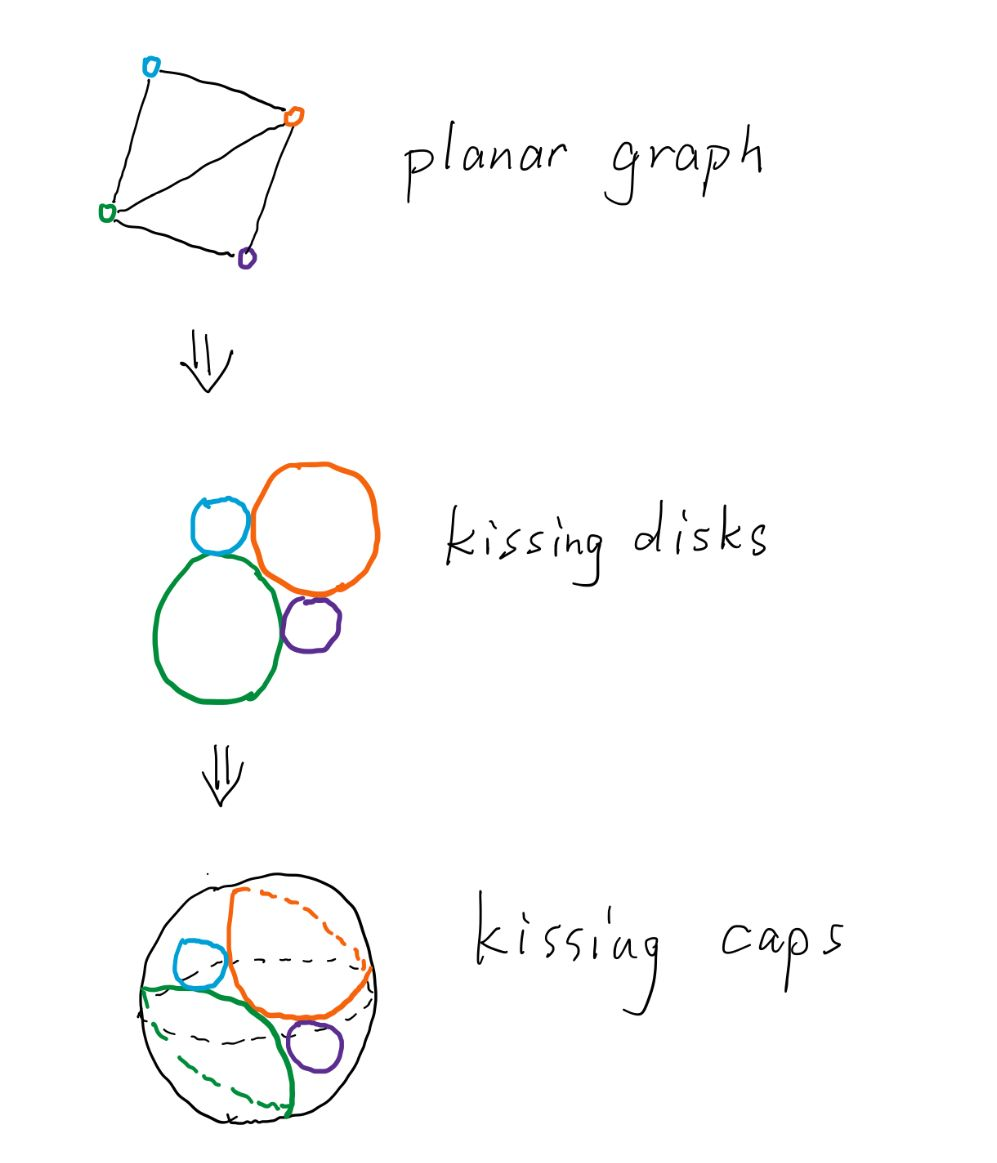
\includegraphics[width=0.5\textwidth]{figures/kissingcaps.jpg}
% \caption{The mapping from planar graphs to kissing disks and kissing caps}
% \label{fig:kissingcap}
% \end{figure}

% \begin{figure}
% \centering
% 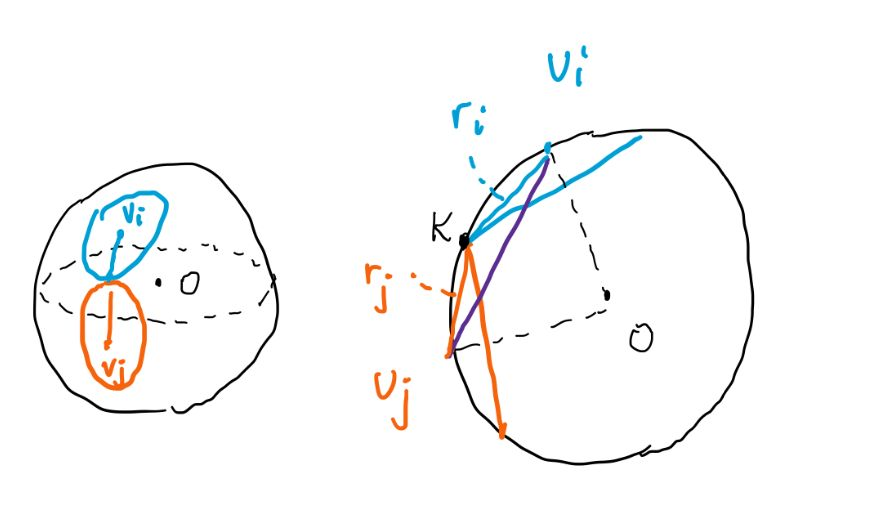
\includegraphics[width=0.5\textwidth]{figures/caps.jpg}
% \caption{The distance between the centers of two kissing caps}
% \label{fig:kissingcap}
% \end{figure}

\section{Sphere Preserving Map}\label{planar}

\begin{definition}
    Let $B^d$ be the unit ball in $d$ dimensions, $S^d$ be the sphere defining the surface of $B^d$.
    A \textbf{sphere preserving map} from $S^d$ to $S^d$ is a continuous function that sends every low-dimension sphere contained in $S^d$ to a sphere in $S^d$, such that every sphere in $S^d$ has a pre-image under the map that is also a sphere. 
\end{definition}
We consider the stereographic projection between the plane and the sphere. For any point $\alpha \in S^d$, we define $\Pi_\alpha$ to be the stereographic projection from the plane perpendicular to $S^d$ at $\alpha$, and let $\Pi_\alpha^{-1}$ be its inverse. We could show that these two functions are sphere-preserving maps \cite{HCV52}.

We then could obtain sphere-preserving maps in the sphere by applying a projection onto a plane, then dilation of the plane, and then mapping back by stereographic projection. For $\alpha \in S^d$ and $a \geq 0$, we define $D^a_\alpha$ to be the map that dilates the hyperplane perpendicular to $S^d$ at $\alpha$ by a factor $a$. 

As the composition of sphere-preserving maps is also a sphere-preserving map, we now define the sphere-preserving map we will user. For any $\alpha$ such that $\|\alpha\|<1$, define $f_\alpha(z)$ by 
\begin{align*}
    f_\alpha(z) = \Pi_{\alpha/\|\alpha\|}(D_{\alpha/\|\alpha\|}^{1-\|\alpha\|}(\Pi_{\alpha/\|\alpha\|}^{-1})(z))
\end{align*}



% \begin{figure}
% 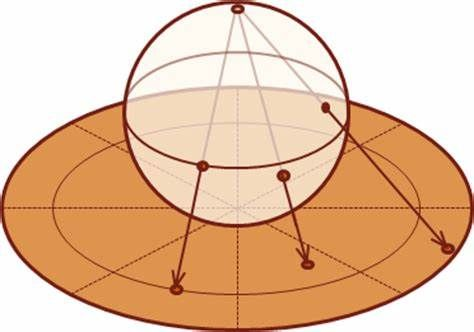
\includegraphics[width=0.4\textwidth]{figures/stereographic.jpg}
% \end{figure}

% A sphere preserving map could be constructed using $\Pi \circ D \circ \Pi^{-1}$, where D is a dilation function


\begin{definition}
    An arrangement of caps ${C_1, ..., C_n}$ in $S^d$ is well-behaved if there is no point that belongs to at least half of the caps.     
\end{definition}
\begin{remark}
    All of the arrangements of caps obtained from graphs contained in the other sections of this report are well-behaved. Otherwise, the induced graphs would have cliques on half o their vertices and no small separators.
\end{remark}

\begin{lemma}
    Let $\phi: B^d \rightarrow B^d$ be a continous function such that, for all $\alpha \in S^d$, $\phi(\alpha)$ lies on the line cnnecting $\alpha$ with $\vzero$ and is closer to $\alpha $ than to $-\alpha$, then there  exists an $\alpha \in B^d$ such that $\phi(\alpha)=\vzero$.  
\end{lemma}\label{le:alpha_exists}
\begin{proof}
We could prove this via contradiction. Assume that there is no point $\alpha \in B^d$ that satisfies $\phi(\alpha)=\vzero$. Consider the map $b(\phi(\alpha))=\phi(\alpha)/\|\phi(\alpha)\|$ with the domain being $B^d - \{\vzero\}$. Since $b$ is a continuous map, $b \circ \phi$ is also a continuous map from $B^d$ onto $S^d$ which is the identity on $S^d$. Therefore, $g(z) = -b(\phi(z))$ is a map from $B^d$ onto $S^d$ that has no fixed point, which contradicts the Brouwer's Fixed Point Theorem, saying that every continuous map from $B^d$ to $B^d$ has a fixed point. 
\end{proof}

With this Lemma, now we could show that we can always find an $\alpha$ and its corresponding map on caps so that the centroid of the centers of their images is at the origin. 

\begin{theorem}
    For any well-behaved arrangement of caps ${C_1, ..., C_n}$ in $S^d$, there is a sphere-preserving map $f_\alpha$ such that the centroid of the centers of $f_\alpha(C_1),f_\alpha(C_2),...,f_\alpha(C_n)$
\end{theorem}\label{th:sum_is_origin}

\begin{proof}
We want to show that there is an $\alpha$ that $\|\alpha\| < 1$ and $\sum_{i=1}^{n}p(f_\alpha(C_i))=\vzero$.
Consider the map from $\alpha$ to the centroid of $\{p(f_\alpha(C_1)), p(f_\alpha(C_2)), ..., p(f_\alpha(C_n))\}$, we want to show that $\vzero$ has a pre-image under this map.

However, the map is not continuous, as when $\|\alpha\| =1$, $-\alpha$ crosses the boundary of $C_i$, and $p(f_\alpha(C_i))$ jumps from one side of the sphere to the other. 

In order to fix this, we construct a modified map that is continous, As the set of caps is well-behaved, we can choose an $\epsilon > 0$ such that for all $\alpha$ that $\|\alpha\| \geq 1-epsilon$, most of the caps $\{(f_\alpha(C_1), f_\alpha(C_2), ..., f_\alpha(C_n)\}$ are entirely contained within the ball of radius $1/2n$ around $\alpha /\|\alpha\|$. As a result, $f_\alpha$ does not map the centroid of the centers of the caps to the origin. For $\alpha \in B^d$, we could define the map as 
\begin{align*}
    \phi(\alpha) = \frac{\sum_{i=1}^{n}w(C_i,\alpha)p(f_\alpha(C_i))}{n}
\end{align*}
where the weight function is 
\begin{align*}
    w(C, \alpha) =  \begin{cases} 
      (2-d(\alpha,C))/\epsilon & d(\alpha,C)\geq 2-\epsilon \\
       1 & otherwise 
   \end{cases}
\end{align*}
The $d(\alpha,C)$ here represents the greatest distance from $\alpha$ to a point in the cap $C$. Since $w$ here is a continuous function that goes to zero as $-\alpha$ approaches the boundary of a cap, $\phi(\alpha)$ is also a continuous function.  

Since we know that $\{C_1, ..., C_n\}$ is well-behaved, it is easy to verify that, for $\alpha \in S^d$, $\phi(\alpha)$ lies on the line connecting $\vzero$ to $\alpha$ and is closer to $\alpha$ compared with $-\alpha$. By Lemma~\ref{le:alpha_exists}, we can find a $\alpha$ such that $\phi(\alpha)=\vzero$.
\end{proof}
% \section{Sphere-Preserving mapping}
% \section{Well-Shaped Meshes}

\bibliographystyle{plainnat}
\bibliography{ref.bib}

\end{document}
